\chapter{Active Media and Radiation}
While the previous chapter dealt with the modelization
of passive dielectric structures, this one will attempt
to model more complex classes of structures. 

The first part will
deal with active dielectric cavities. A recently formulated
steady state \textit{ab initio} laser theory (SALT) solves the 
Schrödinger-Bloch state equations in such a way that the effect of
the active medium can be considered as a pump-dependent
deformation of the refractive index profile. We present a summary 
of the theory and two methods of solution, one based on the phase
accumulated by incoming waves and the other based on Green's
function. 

The second part describes the modelization attempts
of the author on the leaky coax antenna. 
\todo[inline]{More detail}

\section{Lasing and Scattering}
A recently formulated laser theory, named the 
\gls{salt} and developed by A. D. Stone's group
at Yale, has been shown to be an accurate model 
of the light-matter interaction involved in bidimensional
microlasers. Its steady-state nature allows us to apply
the formalism developed in the previous section 
to the theory. However, in light of the several shortcomings
of the \gls{sqa}'s numerical implementation, we have studied 
two other numerical methods. The first one is based on 
differential equations and shares some of the problems of 
the onion method, but has a nice physical interpretation
in terms of phases and is more easily generalizable to 
3D scattering. The other one is based on integral methods 
and seems to be more stable than the other methods.

\subsection{Primer on Steady State ab initio Laser Theory (SALT)}
Our exposition of \gls{salt} will be divided into two main sections:
the first will descrive the details of the interaction of light with
the quantum gain medium and provide a steady-state solution
of the resulting Maxwell-Bloch equations. The second
will discuss the constant-flux states and their computation
using the aforementioned numerical methods. 

\paragraph{Solving the Matter Equations}

\paragraph{Constant-flux States and Scattering}    

\subsection{Methods of Solution}
\paragraph{Variable Phase Method}
\paragraph{Green's Function Method}
\todo[inline]{Primer on VPM for bidimensional cavities (mention its
	      use for 3D cavities with vector spherical wave functions).}
\todo[inline]{Motivation for VPM: computing the field more efficiently than in SQA.}

\section{Smart Textile Antennae}
\subsection{Basic Antenna Theory and HFSS Simulations}
Even today, a full 140 years after the publication of 
Maxwell's \textit{Treatise on Electricity and Magnetism}, 
the electromagnetic modeling of radiating structures 
is an ongoing research problem. The notorious difficulty 
of solving Maxwell's equations seriously hampers analy\-ti\-cal efforts
and, due to the nature of electromagnetic radiation, numerical
progress is not easier to achieve.

In what follows, we present the basic equations of 
antenna theory (Maxwell's) and discuss the nature 
of sources in this framework (currents and charges). 

\subsubsection{Maxwell's Equations}
Being, by now, comfortable with the basic form of Maxwell's equations, 
we will simply state them for linear, non-chiral and reciprocal media
and allow for the existence of current and charge densities. 
They are (in Lorentz-Heaviside units with $c=1$) \cite{NOV2012}
  \begin{subequations}
  \begin{align}
   \nabla\times\bo{E}+\frac{\partial(\mu\bo{H})}{\partial t}	&=0	\\
   \nabla\times\bo{H}-\frac{\partial(\epsilon\bo{E})}{\partial t}-\bo{J}_c&=\bo{J}_s\\
   \nabla\cdot(\epsilon\bo{E})					&=\rho	\\
   \nabla\cdot(\mu\bo{H})					&=0
  \end{align}
  \end{subequations}
where we have separated the current using two terms: a source current, $\bo{J}_s$ and
an induced conduction current $\bo{J}_c$. The induced conduction current
is related to the electric field via Ohm's law, i.e.
  \begin{equation}
   \bo{J}_c=\sigma\bo{E}
  \end{equation}
while the source current is a prepared, physical source initially 
independant of the system.

A technical point is in order. In the antenna literature, the induced
currents and charge density are considered as the fundamental quantities 
that \textit{produce} the fields. While worthwhile (see the Stratton-Chu section), 
this viewpoint requires that either (i) we have \textit{a priori} knowledge of 
the sources ($\bo{J}_t=\bo{J}_c+\bo{J}_s$ and $\rho$) or (ii) that we use the
constitutive relations down the line. The first case applies to situations
where the induced current is trivially known (e.g. the dipole antenna) or
when $\sigma=0$ and $\bo{J}_s$ is known.

Also, even though the $\bo{H}$ field was introduced as an auxiliary field to take
into account the effect of an applied magnetic field to the material, we 
take it as the fundamental field as it leads to more easily solvable
equations and is a completely equivalent choice. 

\subsubsection{Stratton-Chu Solution}
In antenna problems, we want to compute the field values as a function of 
the sources that contribute to these fields. From electrostatics, we know 
that a current density $\bo{J}$ gives rise to an electric field and a charge 
density $\rho$ gives rise to a magnetic field. In the time-varying picture, 
the electric and magnetic fields become coupled and we take the viewpoint that
the $\bo{J}$ and $\rho$ give rise to both electric and magnetic fields. 

To compute the field from these sources, which are presupposed to exist, 
we must use the Stratton-Chu integrals. The derivation is standard, so we 
refer to \cite{ELL2003}. Consider a volume $V$ of free space containing
sources and possibly excluded subvolumes $V_i$ bound by surfaces $S_i$ that contain matter
of some kind. By the use of Green's and Stokes' theorems and other vectorial 
identities, we find that the field outside the excluded subvolumes
can be expressed as
  \begin{align}
   \bo{E} &= \frac{1}{4\pi}\mathop{\iiint}_V \left(\rho\nabla G+i\omega G\bo{J}\right)dV
	+\frac{1}{4\pi}\oiint_{S_1,\cdots,S_N}\left[\bo{n}\cdot\bo{E}\nabla G+(\bo{n}\times\bo{E})\times\nabla G+i\omega G(\bo{n}\times\bo{H})\right]dS\label{eq:antenna.strattonChuE}\\
   \bo{H} &= \frac{1}{4\pi}\mathop{\iiint}_V \bo{J}\times\nabla G dV
	+\frac{1}{4\pi}\oiint_{S_1,\cdots,S_N}\left[-i\omega G(\bo{n}\times\bo{E})+(\bo{n}\times\bo{H})\times\nabla G+(\bo{n}\cdot\bo{H})\nabla G\right]dS\label{eq:antenna.strattonChuH}
  \end{align}
where $G$ is the Green's function of the problem
  \begin{equation}
   G(\bo{r},\bo{r}') = \frac{e^{ik|\bo{r}-\bo{r'}|}}{4\pi|\bo{r}-\bo{r}'|}.
  \end{equation}

These two equations are rigorous solutions of Maxwell's equations. 
They can be used with any antenna and provide ways to compute the 
current distribution if is unknown (constitutes an integral equation in the current)
and can be used to compute the far-field of antennae when either 
(i) the current distribution is known or (ii) the near-field around the antenna
is known. 
These two properties discriminate antennae into two categories, denoted Type I and Type II.

Type I antennae have a well-approximated current distribution, which means that there are no
subvolumes to be excluded and therefore no surface integrals in expressions 
\eqref{eq:antenna.strattonChuE} and \eqref{eq:antenna.strattonChuH}. 

On the other hand, Type II antennae have well-approximated near-fields, leading
us to exclude the volume containing the antenna. Expressions \eqref{eq:antenna.strattonChuE}
and \eqref{eq:antenna.strattonChuH} contain only surface integrals, then. 

\subsubsection{Antenna Parameters}
In the design of our antenna, we will want to optimize the value
of some parameters. We will now describe some of these parameters.

\paragraph[Directivity and Gain]{Directivity and Gain \cite[\S 1.16]{ELL2003}}
Given a radiation pattern measured (in the far-field) as the power density 
$\mathcal{P}(\theta,\varphi)$, we can define its \textit{directivity}
as
  \begin{equation}
   D(\theta,\varphi) = \frac{4\pi\mathcal{P}(\theta,\varphi)}
			{\int_0^\pi\int_0^{2\pi}\mathcal{P}(\theta',\varphi')\sin\theta'd\theta'd\varphi'}.
  \end{equation}
The value of the directivity is less than unity if the power density radiated at angle $(\theta,\varphi)$
is less than the average power radiated. For instance, an isotropic antenna will possess a unit directivity
for all angles while a highly directional antenna will have a sharp peak  in its directivity function 
at some angle $(\theta,\varphi)$.

Another interesting concept to introduce is \textit{partial directivity}. 
The power density can be divided into two contributions: the $\theta$-polarized
and the $\varphi$-polarized polarization and we can write
  \begin{equation}
    \mathcal{P}(\theta,\varphi) = \mathcal{P}_\theta(\theta,\varphi)+\mathcal{P}_\varphi(\theta,\varphi)
  \end{equation}
where the subscripts indicate the polarization state. The partial 
directivities hence follow
  \begin{equation}
   D(\theta,\varphi) = D_\theta(\theta,\varphi)+D_\varphi(\theta,\varphi).
  \end{equation}

We can also introduce the gain, which characterizes the loss
and the directivity of the antenna simultaneously. It is simply given
as
  \begin{equation}
    G(\theta,\varphi) = \frac{4\pi r^2\mathcal{P}(\theta,\varphi)}{P}
  \end{equation}
where $P$ is the power accepted by the antenna. Because of the 
losses, $P/r^2>\int_0^\pi\int_0^{2\pi}\mathcal{P}(\theta',\varphi')\sin\theta'd\theta'd\varphi'$
such that $G(\theta,\varphi)<D(\theta,\varphi)$. 

We can also define partial gains in the exact same fashion we defined partial
directivities.

Radiation efficiency $\eta$ is defined as the ratio of the total radiated power 
to the power accepted by the antenna \cite{IEEE145-1993}.

\paragraph{Scattering Parameters}
The scattering parameters (or $S$-parameters) are
usually defined through a linear $N$-port network. 
Suppose we have an electronic device comprising
$N$ ports, or points of entry. Imagine shining light onto
one of the ports, say port $j$. A certain percentage
of the power carried by this light be reflected 
by this port and the rest will be transmitted to the
other ports or absorbed in the medium. The \textit{reflection}
coefficient is given by $S_{jj}$ while the transmission
coefficients are given $S_{ji}$ ($i\neq j$) where $\mat{S}$
is the scattering matrix of the network. In a reciprocal (in the sense
of Lorentz) network, the scattering matrix will be equal to its
transpose, i.e. $S_{ij}=S_{ji}$. In a lossless network, the scattering
matrix will be unitary. 

This is, of course, highly reminiscent of the scattering operator
in quantum-mechanical scattering which relates the outgoing (scattered)
components to the incoming (incident) components
  \begin{equation}
   \Ket{\Psi_\text{out}}=\mathcal{S}\Ket{\Psi_\text{in}}.
  \end{equation}
In this case, the ``ports'' are the different angular momenta
components rather than physical input/output connections. 
Ports are somewhat arbitrary in optical structures.

\subsection{HFSS Simulations of an LCX Antenna}
In our quest of finding a fibre-antenna design that can easily be integrated into
textile, we have stumbled upon the leaky coaxial cable (LCX) design: a basic coaxial cable
from which are cut windows as to expose the dielectric core. The radiation characteristics
can be tuned by changing the geometric properties of the windows. 

LCX antennae are usually analyzed using harmonic analysis \cite{WAN2001}. 
In our case, however, we cannot consider the structure to be periodic, as the total 
length of the fibre-antenna is of the order of the wavelength ($\lambda\sim12\unit{cm}$) and the period
of the slots is smaller than the wavelength. Moreover, given the size of the slots, 
the author is comfortable to say that we neither are in the perturbation regime. 
Figure \ref{fig:antenna.fibre-antenna} shows the actual design and the important parameters.

Given the wild scale in the size of the structures (from the nanometer to the millimeter), we use
the FEM to solve the driven problem. The parameters of interest will be the scattering parameters, the
radiation pattern and antenna efficiency, gain and directivity. We will first model the fibre-antennae
that were fabricated. There will be a subsequent optimization phase.

\subsubsection{Preliminary Results}
We first model the RF21 design. Its parameters are summarized in 
Table \ref{tab:antenna.rfxx-parameters}. 

Notice the small thickness
of the silver layers (126 and 101 nm) compared to the other 
sizes involved. It takes a highly non-uniform mesh to model
these small relative sizes. Moreover, since the silver has a high
conductivity, it takes an even smaller mesh to model. Our first 
attempts at modeling this structure proved unsuccessful.

In the experimental data (\see Figure \ref{fig:antenna.sParameters}), 
we see deep dips in the transmission spectrum ($S_{12}$) at approximately
1.8 GHz and 3 GHz. There are corresponding dips in the reflection parameters,
$S_{11}$ and $S_{22}$, which leads us to believe that remaining power 
was radiated through the slots. The existence of two dips seems predicated on the asymmetry
of the fibre ($d_L\neq d_R$). 

We also notice that the simulation data does not in any way correlate
to the experimental data. This is probably due to the fact that, in the our
HFSS model, we had to put the thickness of the silvers layers to $2\,\unit{\mu m}$
instead of the values listed in Table \ref{tab:antenna.rfxx-parameters}. In 
this regime, the fibre-antenna behaves like an ordinary transmission line. 
However, as the mesher does not allow us to go under $2\,\unit{\mu m}$, we cannot
conclude that is really due to the thickness of the Ag layers, only suspect it.

In our following report, we will break down the problem
to make it analytically tractable and try to analyze the effect of ``small''
silver layers on the propagation of light. 

\begin{figure}
 \begin{center}
 \begin{tikzpicture}
  % -- Draw the overall shape.
  \draw[very thick] (0,0) -- (8,0) -- ++(0,-2) -- ++(-3,0) -- ++(0,-2) -- ++(-2,0) -- ++(0,2) -- ++(-3,0) -- ++(0,2); 
  
  % -- We draw the reflected/transmitted arrows.
  \draw[->,>=stealth] (8.25,-0.5) -- ++(1,0) node[near end,above] {$a_1$};
  \draw[<-,>=stealth] (8.25,-1.5) -- ++(1,0) node[near end,above] {$b_1$};
  \draw[<-,>=stealth] (-1.25,-0.5) -- ++(1,0) node[near start,above] {$a_2$};
  \draw[->,>=stealth] (-1.25,-1.5) -- ++(1,0) node[near start,above] {$b_2$};
  \draw[->,>=stealth] (3.5,-4.25) -- ++(0,-1) node[near end,right] {$a_3$};
  \draw[<-,>=stealth] (4.5,-4.25) -- ++(0,-1) node[near end,right] {$b_3$};
 \end{tikzpicture}
 \end{center}
 \caption[Example of a 3-port network]{Example of a 3-port network. The ``ends'' of the structure are generally used at its ports.}
 \label{fig:antenna.network}
\end{figure}

\begin{figure}
 \centering
 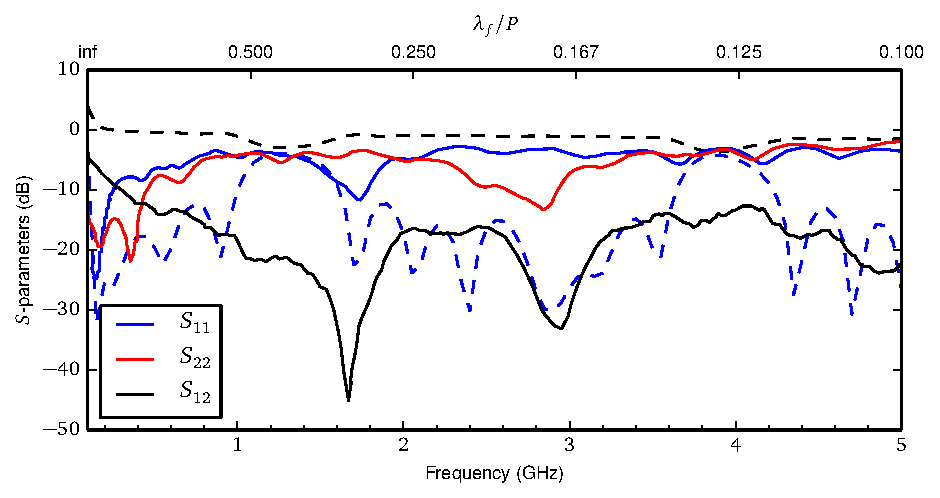
\includegraphics[width=\textwidth]{figs/active/sParametersRF21.pdf}
 \caption[$S$-parameters of the RF21 fibre design]{$S$-parameters of the RF21 fibre design. The full lines represent
	  the experimental data while the dotted lines represent the simulation data.
	  The top $x$ axis shows the $S$-parameters as a function of the ratio of the 
	  vacuum wavelength $\lambda_f$ over the period of the windows $P$.}
 \label{fig:antenna.sParameters}
\end{figure}


\begin{figure}
 \centering
 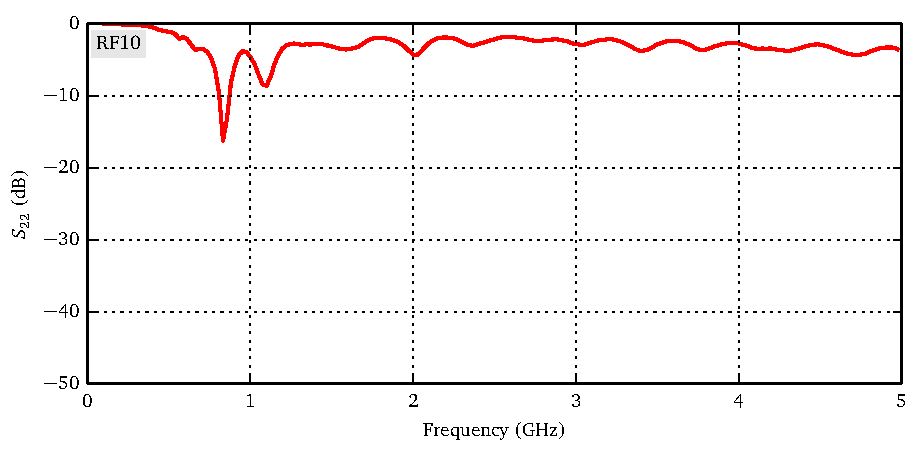
\includegraphics{figs/active/RF10-sParameters.pdf}
 \caption{$S$-parameters of ...}
\end{figure}

\begin{figure}
 \centering
 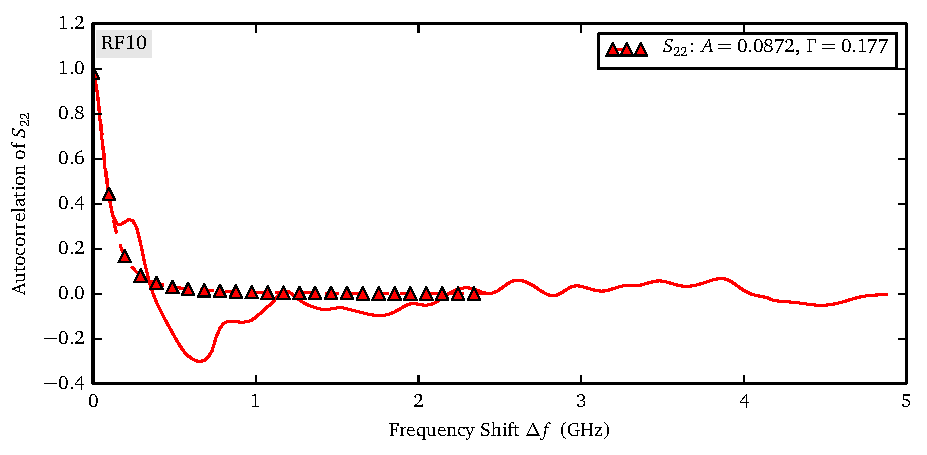
\includegraphics{figs/active/RF10-autoCorrelation.pdf}
 \caption{Autocorrelation of ...}
\end{figure}

\begin{figure}
 \centering
 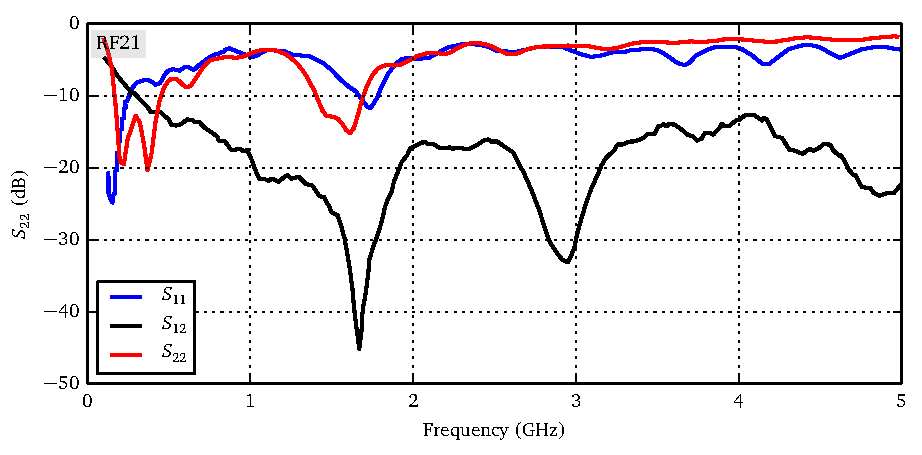
\includegraphics{figs/active/RF21-sParameters.pdf}
 \caption{$S$-parameters of ...}
\end{figure}

\begin{figure}
 \centering
 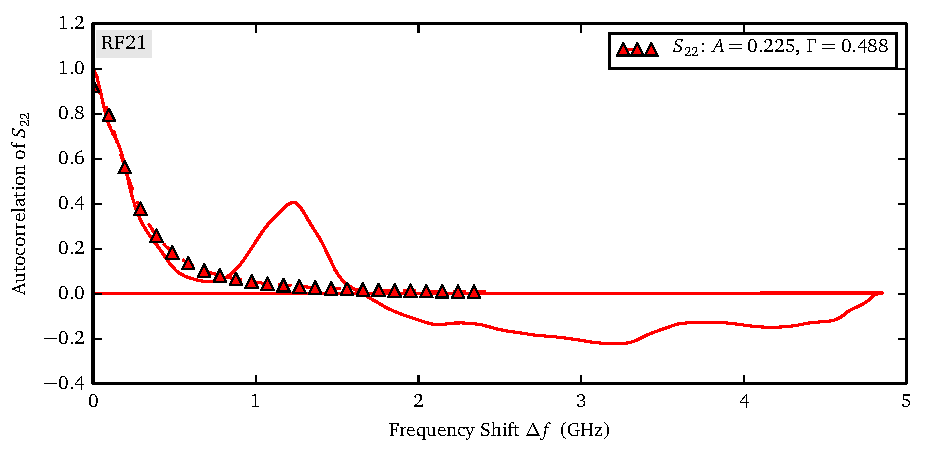
\includegraphics{figs/active/RF21-autoCorrelation.pdf}
 \caption{Autocorrelation of ...}
\end{figure}

\begin{figure}
 \centering
 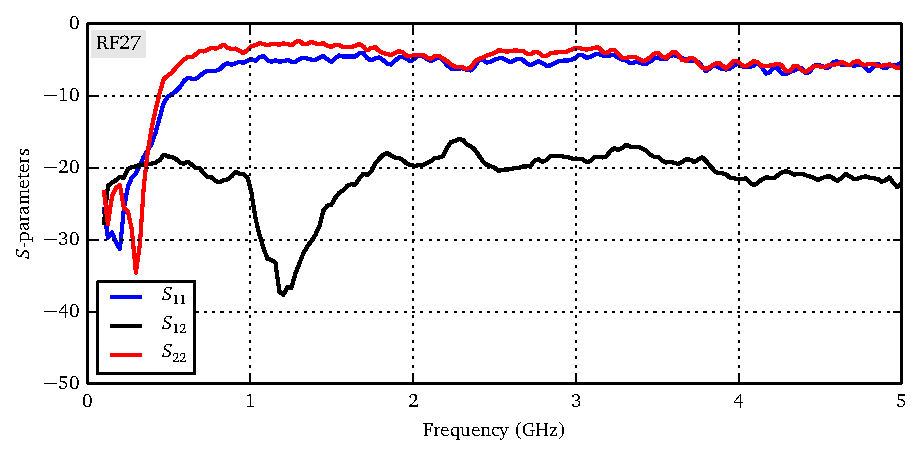
\includegraphics{figs/active/RF27-sParameters.pdf}
 \caption{$S$-parameters of ...}
\end{figure}

\begin{figure}
 \centering
 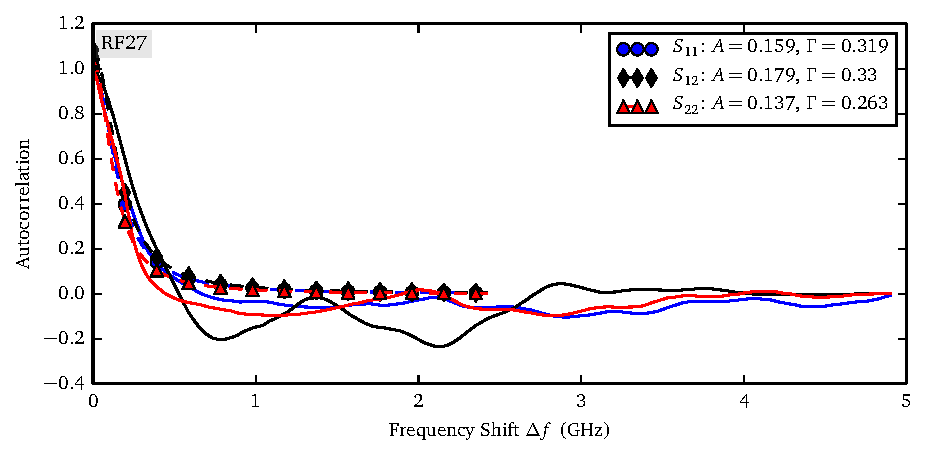
\includegraphics{figs/active/RF27-autoCorrelation.pdf}
 \caption{Autocorrelation of ...}
\end{figure}

\begin{figure}
 \centering
 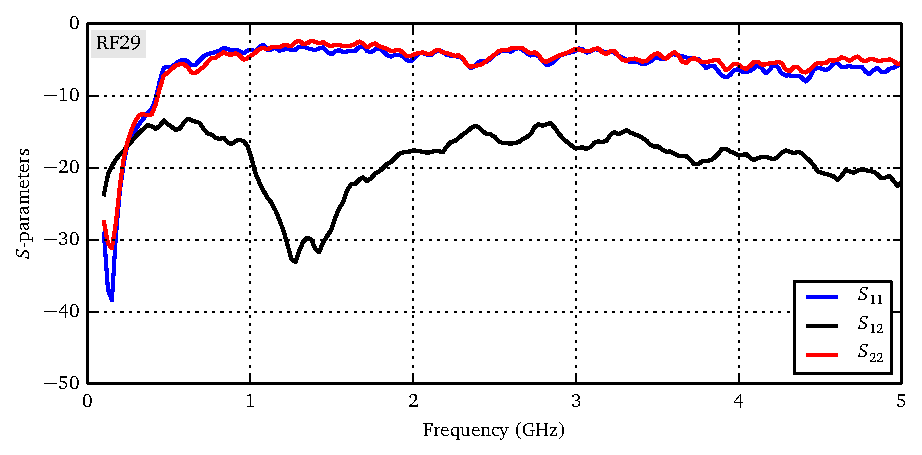
\includegraphics{figs/active/RF29-sParameters.pdf}
 \caption{$S$-parameters of ...}
\end{figure}

\begin{figure}
 \centering
 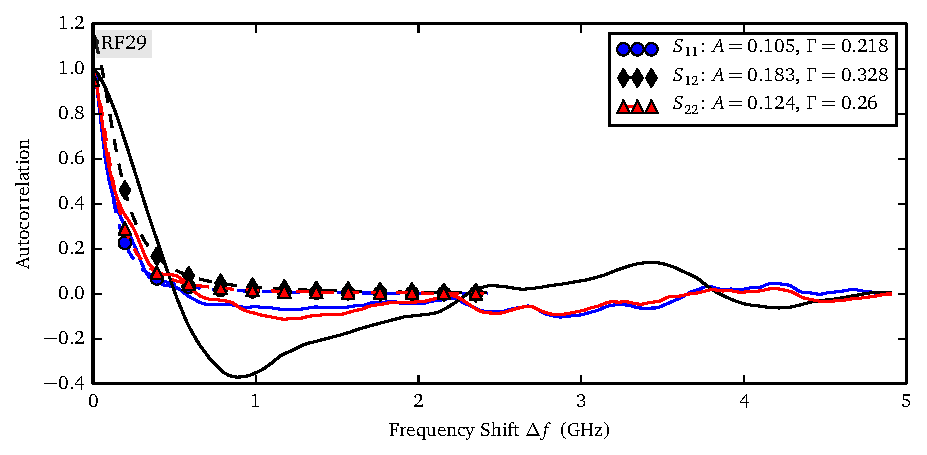
\includegraphics{figs/active/RF29-autoCorrelation.pdf}
 \caption{Autocorrelation of ...}
\end{figure}

\begin{figure}
 \centering
 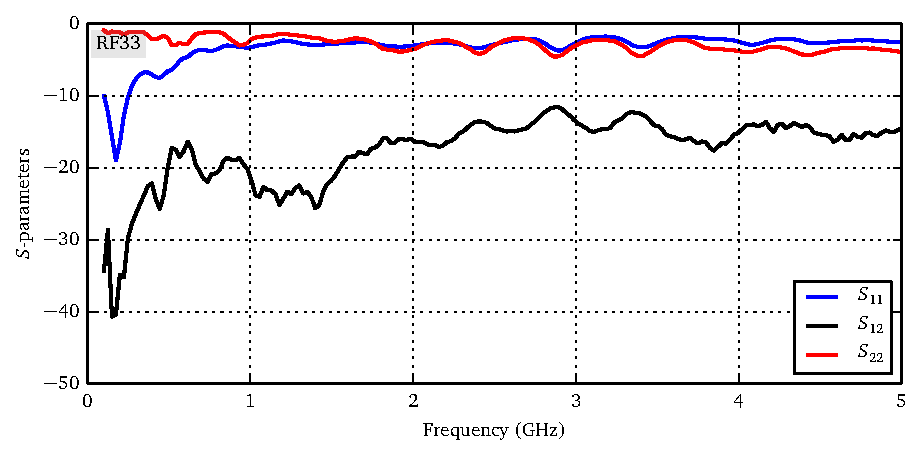
\includegraphics{figs/active/RF33-sParameters.pdf}
 \caption{$S$-parameters of ...}
\end{figure}

\begin{figure}
 \centering
 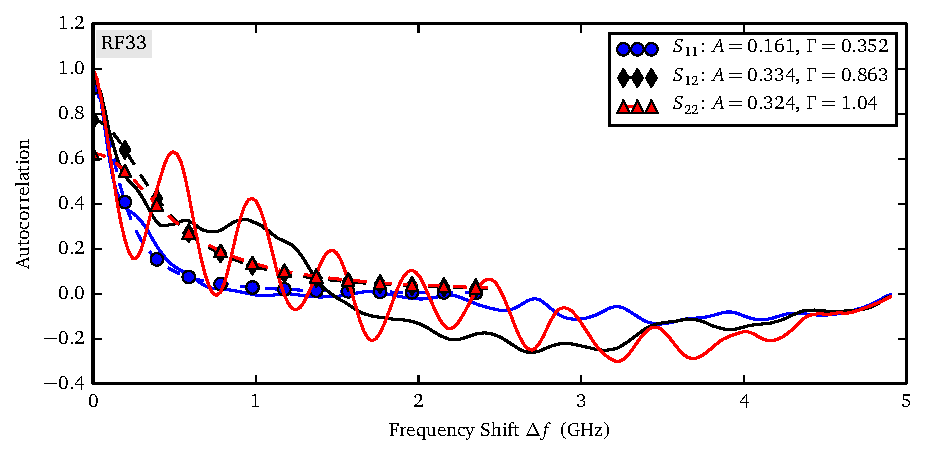
\includegraphics{figs/active/RF33-autoCorrelation.pdf}
 \caption{Autocorrelation of ...}
\end{figure}

\begin{figure}
 \centering
 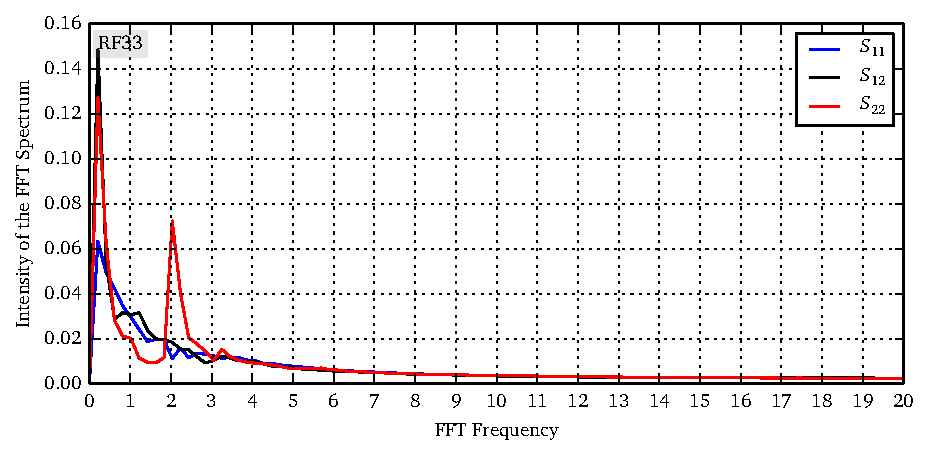
\includegraphics{figs/active/RF33-fft.pdf}
 \caption{FFT of ...}
\end{figure}

\section{Antenna Modelization}
The goal of this project is to develop an antenna that is compatible with 
WiFi standards (i.e. emits at $f=2.45\,\unit{GHz}$) and easily integrated
to textile. These two requirements impose multiple restrictions on both
the materials that can be used and the geometry of the antenna. For seamless
integration, we would like the antenna to be spun directly into the textile. 

Most solutions today merely affix a patch antenna to a less 
encumbered part of the textile, e.g. on the should pads of a shirt
or the front of a t-shirt.
A metallic plate shields the user from the electronic components 
of the patch antenna. Because the properties of patch antennas are
well known, it requires very little engineering and is thus cheap. However, integration 
with the textile is far from seamless, as it is very apparent to the
user that he has become a giant walking antenna. Our project thus 
strives to find antenna designs that have emission properties
as flexible as a patch antenna's while improving textile integration
as to make it become transparent to the user.

The concept of a fibre-antenna rapidly established itself
as an ideal solution in the research group. It provides a rich
architecture upon which to build. Moreover, it can easily 
be spun into textile as it can loaded into the spools that 
deliver threads to looms. Its mechanical properties make it
fit for daily use as it can resist a trip in the washing machine. 
Integration of the electronic components inside that fibre 
serves to shield both the user and the components. 

\begin{figure}
  \centering
  \begin{subfigure}[b]{\textwidth}
    \centering
   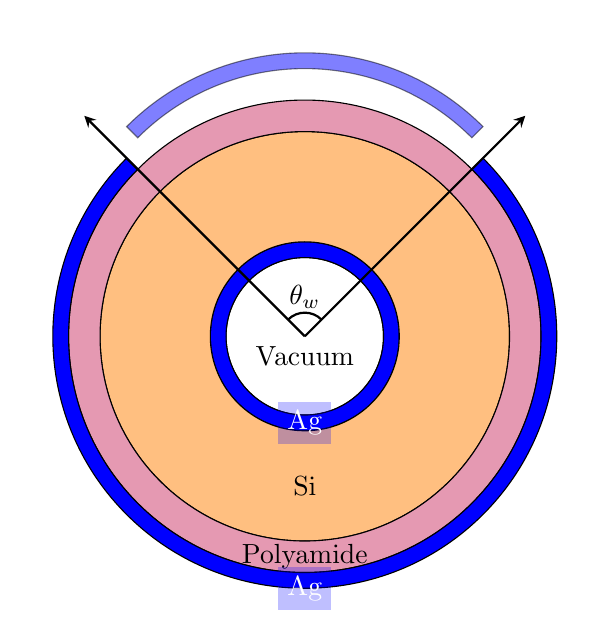
\begin{tikzpicture}
    % -- Draw different materials of the antenna.
    \coordinate (O) at (0,0);
    \draw (O) circle (1);											% Vacuum core
    \draw[fill=blue, even odd rule] (O) circle (1.2) (0:1) arc (0:360:1);					% Silver layer
    \draw[fill=orange!50!white, even odd rule] (O) circle (2.6) (0:1.2) arc (0:360:1.2);			% Dielectric (Si) layer
    \draw[fill=purple!40!white, even odd rule] (O) circle (3) (0:2.6) arc (0:360:2.6);				% Dielectric (polyamide) layer
    \draw[fill=blue,even odd rule] (45:3) -- (45:3.2) arc (45:-225:3.2) -- (-225:3) arc (-225:45:3) -- cycle;	% Second silver layer
    \draw[fill=blue,opacity=0.5,even odd rule,yshift=0.4cm] (45:3) -- (45:3.2) arc (45:135:3.2) -- (135:3) arc (135:45:3) -- cycle;
    
    % -- Draw the angular size of the window.
    \draw[->,>=stealth,thick] (O) -- (-2.8,2.8);
    \draw[->,>=stealth,thick] (O) -- (2.8,2.8);
    \draw[thick] (45:0.3) arc (45:135:.3); 
    \node at (0,0.5) {$\theta_w$};
    
    % -- Place text for materials
    \node at (0,-0.25) {Vacuum};
    \node[text=white,fill=blue,fill opacity=0.25,text opacity=1] at (0,-1.1) {Ag};
    \node at (0,-1.9) {Si};
    \node at (0,-2.8) {Polyamide};
    \node[text=white,fill=blue,fill opacity=0.25,text opacity=1] at (0,-3.2) {Ag};
   \end{tikzpicture}
   \vspace{0.25cm}
   \caption{View of the cross-section: in order of increasing radius, we have: vacuum, silver, silica, polyamide and silver.
	    We have shown a cross-section where there is a ``window''. When there are no windows, 
	    the outer silver layer takes up the entire circumference of the fiber.
	    $\theta_w$ is the angular size of the windows.}
   \label{fig:antenna.fibre-antenna.xsection}
  \end{subfigure}
  
  \vspace{2cm}
  
  \begin{subfigure}[b]{\textwidth}
    \centering
   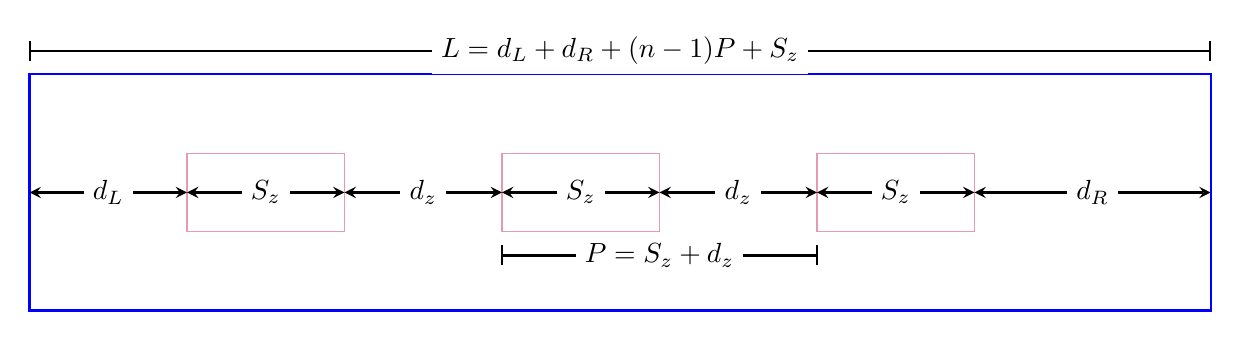
\begin{tikzpicture}
    \draw[blue,thick] (0,-0.5) rectangle (15,2.5);
    \draw[purple!40!white] (2,0.5) rectangle (4,1.5);
    \draw[purple!40!white] (6,0.5) rectangle (8,1.5);
    \draw[purple!40!white] (10,0.5) rectangle (12,1.5);
    
    \draw[<->,>=stealth,thick] (0,1) -- (2,1) node[midway,fill=white] {$d_L$};
    \draw[<->,>=stealth,thick] (2,1) -- (4,1) node[midway,fill=white] {$S_z$};
    \draw[<->,>=stealth,thick] (4,1) -- (6,1) node[midway,fill=white] {$d_z$};
    \draw[<->,>=stealth,thick] (6,1) -- (8,1) node[midway,fill=white] {$S_z$};
    \draw[<->,>=stealth,thick] (8,1) -- (10,1) node[midway,fill=white] {$d_z$};
    \draw[<->,>=stealth,thick] (10,1) -- (12,1) node[midway,fill=white] {$S_z$};
    \draw[<->,>=stealth,thick] (12,1) -- (15,1) node[midway,fill=white] {$d_R$};
    \draw[|-|,thick] (-0.01,2.8) -- (15.01,2.8) node[midway,fill=white] {$L=d_L+d_R+(n-1)P+S_z$};
    \draw[|-|,thick] (5.99,0.2) -- (10.01,0.2) node[midway,fill=white] {$P=S_z+d_z$};
   \end{tikzpicture}
   \vspace{0.25cm}
   \caption{Top view: the positions of the windows are usually asymmetric, i.e. $d_L\neq d_R$. The distance between
	    the windows is given by $d_z$ and the length of the windows are $S_z$. We notice that the length of the 
	    fibre is given by $L=d_L+d_R+(n-1)P+S_z$ where $P=S_z+d_z$ is the period between windows and $n$ is the number
	    of windows.}
   \label{fig:antenna.fibre-antenna.topview}
  \end{subfigure}
  \caption{Geometry of the fibre-antenna}
  \label{fig:antenna.fibre-antenna}
\end{figure}

\subsection{Leaky Coaxial Cable}
The first design we have looked into is a well known one:
the \textit{leaky coaxial fibre} (LCXF). It simply consists of
a coaxial cable (metal rod, dielectric layer, metal coating)
from which we have removed some of the metallic coating. 
These holes in the metallic coating are called ``windows'' and
allow light to escape the confines of the coax cable, hence
the moniker \textit{leaky}. In the following section, we will
look at several methods that we used to model the device
and present the design parameters that were used. 

\subsubsection{Specifications of the Devices}
An image is worth a thousand words. Figure \ref{fig:antenna.fibre-antenna.xsection}
shows a cross-section of the fibre. Figure \ref{fig:antenna.fibre-antenna.topview} 
shows a top view of the antenna and display the positions of the windows. 
Multiple designs have been fabricated, but we retain only those that 
we have tried to simulate. Table \ref{tab:antenna.rfxx-parameters} 
shows the actual geometrical parameters of the fibre-antennas.

\paragraph*{On the thickness of the silver shells}
The thicknesses of the dilectric materials are provided by the manufacturer, 
Polymicro Technologies, safe for the thicknesses of the silver layers. 
For the time being, we have calculated those thicknesses by measuring
the DC resistance of the inner and outer layers of silver and
using the relation \cite[p.~204]{CHE1989}
  \begin{equation}
    \label{eq:antenna.dcResistivity}
    R = \frac{L}{\sigma A}
  \end{equation}
where $L$ is the length of the fibre, $\sigma$ the conductivity of the silver
layer and $A$ its area. For the inner and outer layers, we have
  \begin{align}
    A_\text{inner}	&= \int_0^{2\pi}\int_{t_\text{vac}}^{t_\text{vac}+t_\text{Ag1}}r\,dr d\theta= \pi\left(2t_\text{vac}t_\text{Ag1}+t_\text{Ag1}^2\right)	\\
    A_\text{outer}	&= \int_0^{2\pi}\int_T^{T+t_\text{Ag2}}r\,dr d\theta = \pi\left(2Tt_\text{Ag2}+t_\text{Ag2}^2\right)
  \end{align}
where $T=t_\text{vac}+t_\text{Ag1}+t_\text{Si}+t_\text{pyamide}$. 
Substituting these results into \eqref{eq:antenna.dcResistivity}
yields
  \begin{subequations}
  \label{eq:antenna:thickGeneralEquations}
  \begin{align}  
   t_\text{Ag1}^2 + 2t_\text{vac}t_\text{Ag1}-\frac{L}{\sigma_\text{Ag0}\pi R_\text{inner}}	&=0	\\
   t_\text{Ag2}^2 + 2Tt_\text{Ag2}-\frac{L}{\sigma_\text{Ag0}\pi R_\text{outer}}			&=0
  \end{align}
  \end{subequations}
where the $R$s are the measured D.C. resistances measured for each shell. 
This can readily be solved using the quadratic equation. Using the bulk conductivity
of silver (see Table \ref{tab:antenna.physicalParameters}) yields the 
thicknesses found in Table \ref{tab:antenna.rfxx-parameters}.

In our previous simulations, it was clear that something was amiss:
there was no correlation between the simulation and
experimental data. AFM pictures (see Figure \ref{fig:antenna.AFM})  have suggested that the deposited
metal is in fact a mixture of silver and silver oxide. To evaluate
the effective conductivity of the mixture, we have used Bruggeman's model \cite{LAN1978}.
The model starts from a homogeneous medium, call it medium 1, 
of conductivity $\sigma_1$ and replaces spherical portions of this material 
by another one of conductivity $\sigma_2$. When this process is done, 
we are left with a inhomogeneous material with partial concentrations $\delta_i$
of each material. The effective conductivity $\sigma_e$ of the medium can be computed
using the relation (for an arbitrary number of materials)
  \begin{equation}
    \sum_i^n \delta_i \frac{\sigma_i-\sigma_e}{\sigma_i+(d-1)\sigma_e} =0 
  \end{equation}
where $\sum_i\delta_i=1$ and $d$ is the dimensionality of the system.
Solving for $\sigma_e$ in the case $n=2$ yields
  \begin{equation}
   (d-1)\sigma_e^2+\left[\left(d\delta_1-1\right)\sigma_1+\left(d\delta_2-1\right)\sigma_2\right]+\sigma_1\sigma_2=0.
  \end{equation}
The positive solution is, defining $q=\left(d\delta_1-1\right)\sigma_1+\left(d\delta_2-1\right)\sigma_2$
  \begin{equation}
   \label{eq:antenna:bruggeman}
   \sigma_e = \frac{1}{2d-2}\left[q+\sqrt{q^2+4(d-1)\sigma_1\sigma_2}\right].
  \end{equation}
  
\begin{figure}
 \centering
 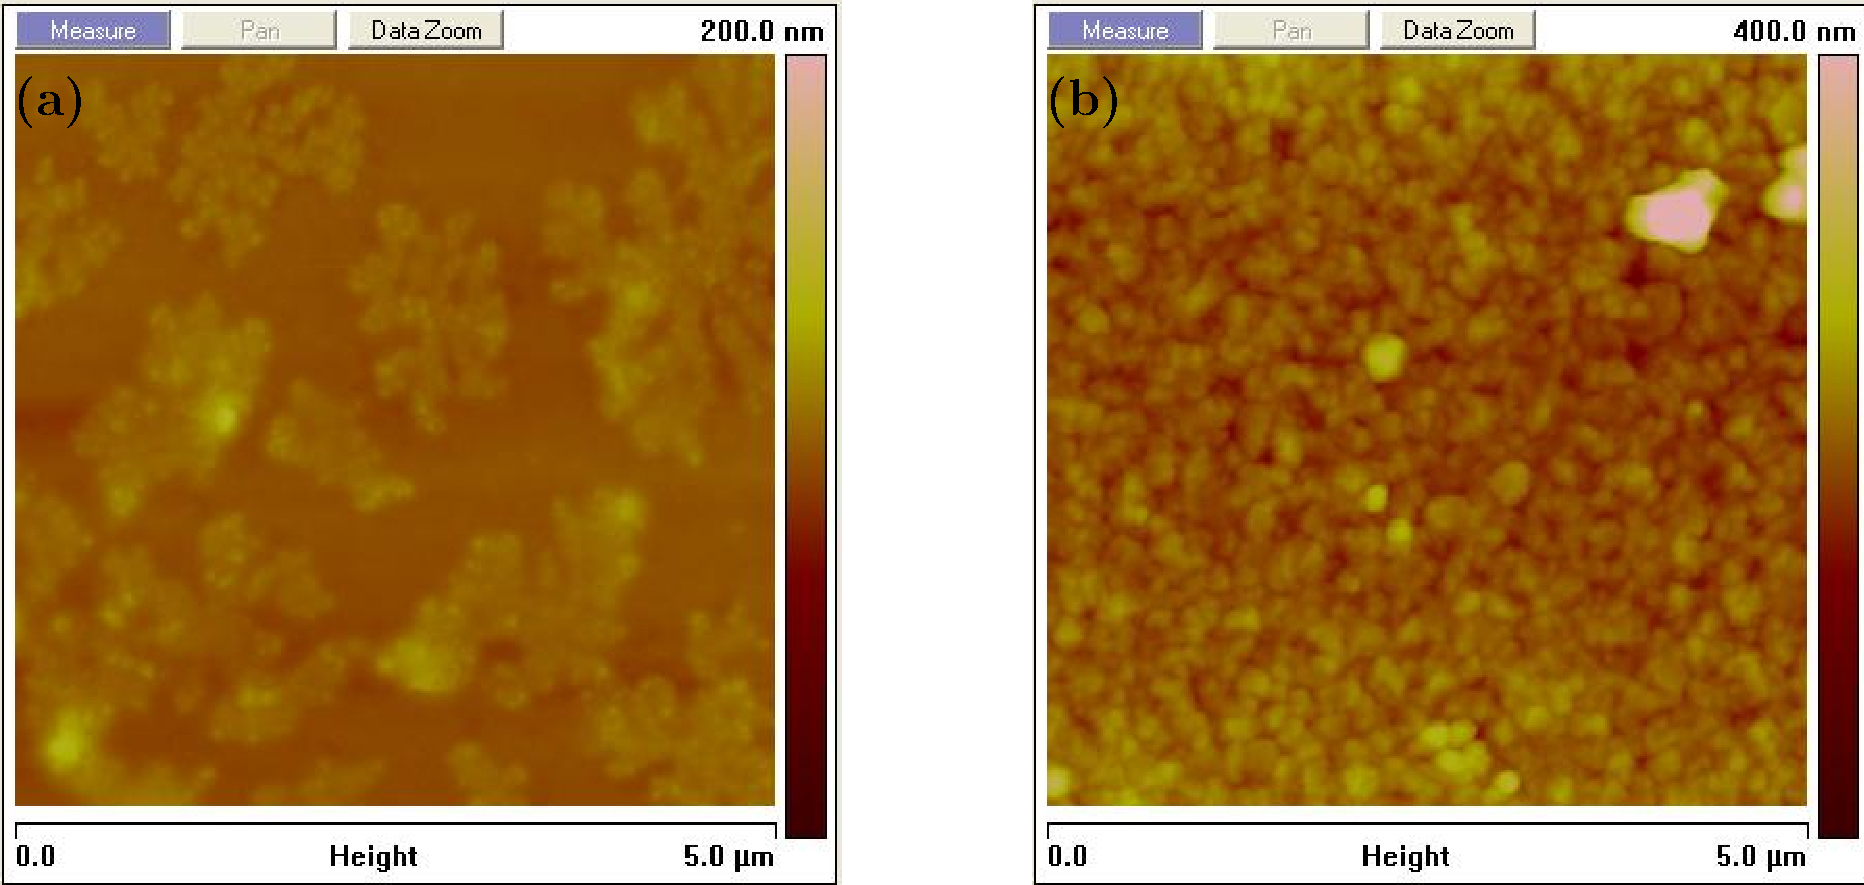
\includegraphics[width=0.8\textwidth]{figs/active/out/AFM.pdf}
 \caption[AFM pictures of silver deposited onto glass plates]{AFM pictures of silver deposited onto glass plates. \textbf{(a)} Flakes of silver oxide seem to be forming onto the deposited
	  silver layer. \textbf{(b)} Sample image showing the inhomogeneity of the
	  silver layer.}
 \label{fig:antenna.AFM}
\end{figure}


\paragraph*{Size Effects}
It has recently come to our attention that the conductivity 
of thin metal films can be a function of their thicknesses. 
We will explore this in future work, so for now 
suffice it to say that the Fuchs-Sondheimer model states
that
  \begin{equation}
      \sigma_F = \frac{\sigma_0}{1+\frac{3\lambda}{8d}\left(1-p\right)}
  \end{equation}
where $0\leq p\leq1$ is a specularity parameter and $\lambda$ is the 
electron free mean path in the metal. This model states that conductivity
diminishes as the thickness of the metallic layer gets smaller.


In Figure \ref{fig:antenna.thicknessRatios}, we compare the 
thicknesses obtained via the bulk conductivity model (Bruggeman 
effective conductivity) and the Fuchs-Sondheimer model with 
effective conductivity for the RF33 fibre. Given that the AFM pictures
show surface inhomogeneity, we assume diffuse scattering in 
the FS model ($p=0$). We see that chosing a dimensionality 
of 3 or 2 does not significantly affect the thicknesses, but
we see a difference of about 20\% in the effective conductivities.

The most interesting thing, though, is that the FS
model predicts metallic layers that are 10\% to 80\% thicker 
than with the bulk conductivity model. This will be explored 
in the next report. 

\begin{table}
  \newcolumntype{d}{D{.}{.}{3}}
  \caption[Geometric and physical parameters of the \gls{lcx} antennae]
	  {Geometric and physical parameters of the \gls{lcx} antennae.
	  Units are repeated from column above if not indicated.}
 \begin{subtable}[t]{0.45\textwidth}
 \caption[Geometric parameters of the RF21/RF33 fibre designs]
	  {Geometric parameters of the RF21/RF33 fibre designs. 
	  The thicknesses of the layers are listed in order, stating
	  from the inner layer to the outer layer of the fibre-antenna.}
 \label{tab:antenna.rfxx-parameters}
 \begin{tabular*}{\textwidth}{l@{\extracolsep{\fill}}c@{\extracolsep{\fill}}d@{\extracolsep{\fill}}d}
  \hline\hline
  Quantity			& Unit			& \multicolumn{1}{c}{RF21} 	& \multicolumn{1}{c}{RF33}	\\
  \hline
  $t_\text{vac}$		& $\unit{\mu m}$	& 99.874			& 99.924			\\
  $t_\text{Ag1}$		& 			& 0.126				& 0.0766			\\
  $t_\text{Si}$			& 			& 273				& 273				\\
  $t_\text{pyamide}$		& 			& 24				& 24				\\
  $t_\text{Ag2}$		& 			& 0.101				& 0.030				\\
  $d_L$				& $\unit{mm}$		& 27				& 30.91				\\
  $d_R$				& 			& 55				& 54.72				\\
  $S_{z1}$\parnote{Each window has a different $S_z$ and $d_z$.}
				& 			& 32				& 34.36				\\
  $S_{z2}$			& 			& 32				& 34.06				\\
  $S_{z3}$			& 			& 32				& 33.87				\\
  $d_{z1}$			& 			& 28				& 27.44				\\
  $d_{z2}$			& 			& 28				& 28.36				\\
  $L$				& $\unit{cm}$		& 30.0				& 24.372			\\
  $\theta_w$			& $\unit{deg}$		& 180				& 180				\\
  $R_\text{inner}$		& $\unit{\Omega}$	& 60.0				& 80.5				\\
  $R_\text{outer}$		&			& 20.0				& 59.8				\\
  \hline\hline
 \end{tabular*}
 \begin{flushleft}
 \parnotes
 \end{flushleft}
 \end{subtable}\hfill
 \begin{subtable}[t]{0.45\textwidth}
  \begin{center}
 \caption{Physical parameters of the materials used in the RF21/RF33 antennas.}
 \label{tab:antenna.physicalParameters}
 \begin{tabular*}{\textwidth}{l@{\extracolsep{\fill}}c@{\extracolsep{\fill}}d}
  \hline\hline
  Quantity			& Unit			& \multicolumn{1}{c}{Value}		\\
  \hline
  $\epsilon_\text{Si}$		& --			& 3.77		\\
  $\epsilon_\text{pyamide}$	& --			& 3.50		\\
  $\sigma_\text{Ag0}$		& $\unitfrac{MS}{m}$	& 63.0		\\
  $\sigma_\text{AgO0}$		& 			&  6.79		\\
  $\lambda_\text{Ag}$		& $\unit{nm}$		& 40		\\
  \hline\hline
 \end{tabular*}
 \begin{flushleft}
 \parnotes
 \end{flushleft}
 \end{center}
 \end{subtable}
\end{table}


\begin{figure}
  \centering
  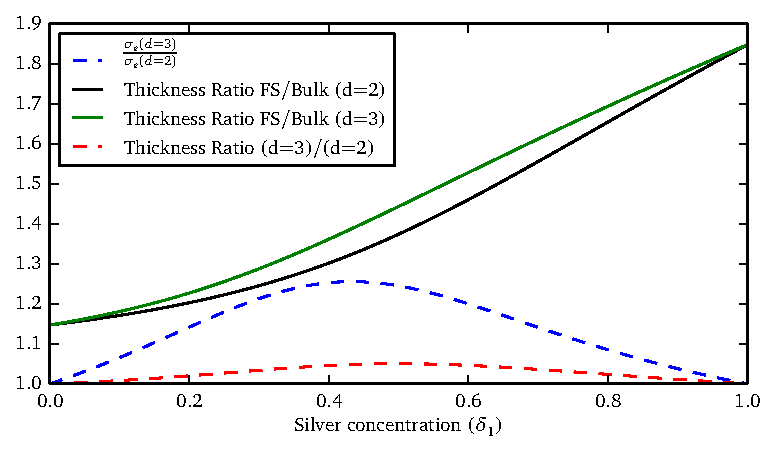
\includegraphics[width=0.9\textwidth]{figs/active/comparisonThickness.pdf}
  \caption[Thickness ratios as a function of the silver concentration]
	  {We show multiple ratios as a function of the silver concentration,
	  $\delta_1$. The blue line shows the ratio between the effective
	  conductivities for a choice of $d=2$ and $d=3$. The black and 
	  green lines show the ratio of the thickness predicted by using
	  the Fuchs-Sondheimer conductivity in Eq. \eqref{eq:antenna:thickGeneralEquations}
	  to the thickness predicted by using the bulk conductivity.
	  The red line shows the ratio of the green line to the black line.}
  \label{fig:antenna.thicknessRatios}
\end{figure}


\subsubsection{Finite Element Method}
As finite element methods directly solve Maxwell's equations, 
they can be a useful tool to verify semi-analytical methods. 
In the last report, we reported some agreement issues 
between experimental and simulation data. We purported
that the discrepancy was due to the small size of the
silver layers that we could properly account for in 
the finite element model. This issue has been solved
by abandoning the idea of properly meshing the silver layers
and replacing them by appropriate impedance boundary conditions.
From HFSS's documentation, we see that the ``Layered Impedance 
Boundary Conditions'' module follows the theory set forth in 
\cite{MIT1968} and others. 

We have simulated the RF21 fibre using Bruggeman's model
for the effective conductivity and with values
of $\delta_1\in\{0,1\}$ and $d=3$ in \eqref{eq:antenna:bruggeman}.
After obtaining the simulated $S_\text{11}$ parameter of the fibre,
we compared it to the experimentally obtained one using the Pearson
correlation coefficient. For two samples $\{X_i\}$ and 
$\{Y_i\}$, it is defined as
  \begin{equation}
    r = \frac{\sum_i^n\left(X_i-\left\langle X\right\rangle\right)\left(Y_i-\left\langle Y\right\rangle\right)}
	     {\sqrt{\sum_i^n\left(X_i-\left\langle X\right\rangle\right)^2}\sqrt{\sum_i^n\left(Y_i-\left\langle Y\right\rangle\right)^2}}.
  \end{equation}
From the definition, we see that the simultaneous linear transformations $X_i\rightarrow b+aX_i$ and $Y_i\rightarrow d+cY_1$
do not change the value of the Pearson coefficient. This means that even if the two samples
do not have the same normalization or are shifted by a constant amount, the correlation 
will stay the same. As such, the Pearson correlation measures the delegend(loc=1, prop={'size':6})
gree at which 
both samples are linearly related. 

Figure \ref{fig:antenna.sParameters} shows the experimental and simulated
$S_{11}$ parameter. At first look, it might seem like the general form 
of the curves are similar, but our quantitative analysis will show 
that that would be wrong. To make sure that our simulation data was not simply
shifted in frequency due to an small error in the geometry, we have
also calculated the correlation for a shifted dataset 
\footnote{To do so, we simply right-shifted the arrays containing
the simulation data and removed the data that fell outside the frequency range 
of the experimental data.}. This changes
the Pearson correlation because we must elide some of the experimental
and simulation data to do so. Figure \ref{fig:antenna.shiftCorrelation}
shows our results. We see that there are little to no correlation
between the simulation data and the experimental data with $r\in\{-0.04,0.05\}$. 

A possible source of error is the thickness of the silver layers. We will incorporate
the FS model in the next simulations and determine if it is
a factor. 

\begin{figure}
 \centering
 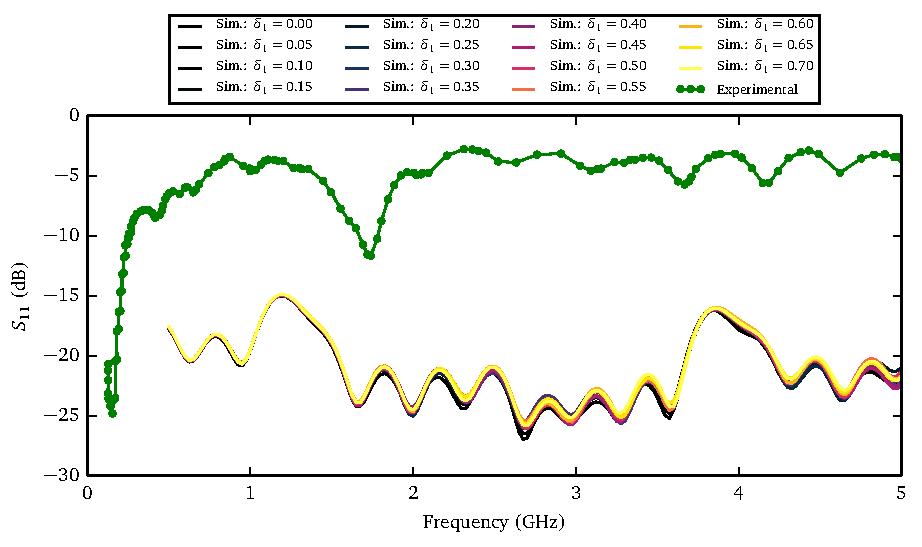
\includegraphics[width=0.8\textwidth]{figs/active/sParameters-concSweepS11.pdf}
 \caption[Experimental and simulated $S_{11}$ parameter for the RF21 fibre]
	 {Experimental and simulated $S_{11}$ parameter for the RF21 fibre.}
 \label{fig:antenna.sParameters}
\end{figure}

\begin{figure}
 \centering
 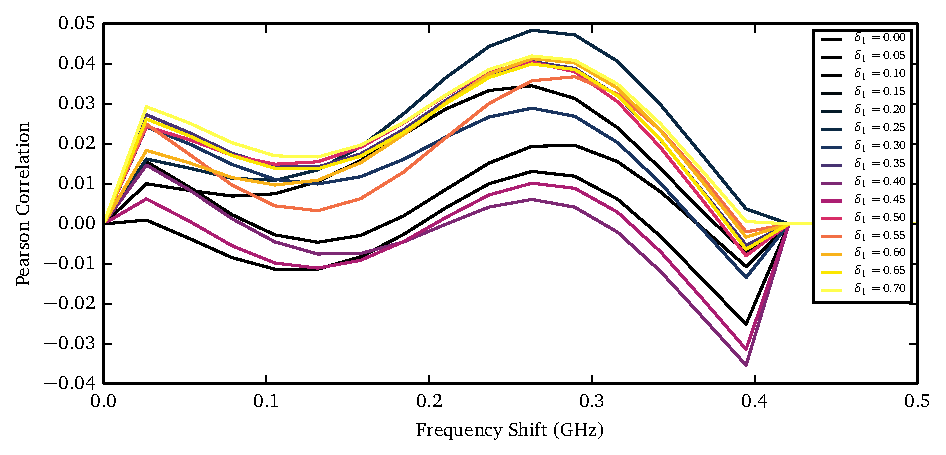
\includegraphics[width=0.8\textwidth]{figs/active/shiftCorrelationS11.pdf}
 \caption{Pearson correlation coefficient as a function of the frequency
	  shift of the data.}
 \label{fig:antenna.shiftCorrelation}
\end{figure}

We have also taken the Fourier transform of the experimental
and simulation data (for $\delta_1=0$). To our discontent, 
it seems that the datasets do not share periodic properties. 
Figure \ref{fig:antenna.fourierAnalysis} shows the intensity
of the FFT transform. To see if the periodic components corresponded
to particular lengths in the system, we converted the associated
wavelenghts to frequencies and plotted them as vertical lines in the figure. 
$f_1$ is the fundamental mode of infinite LCXF, namely
  \begin{equation}
   f_1 = \frac{c}{\left(S_z+d_z\right)\left(\sqrt{\epsilon_\text{Si}}+1\right)}.
  \end{equation}
The frequency associated with the optical and the actual lengths of the window
are
  \begin{align*}
   l_\text{opt}	&= \frac{c}{S_z\sqrt{\epsilon_\text{Si}}}	\\
   l_\text{phy}	&= \frac{c}{S_z}.
  \end{align*}

Nothing thus far seems to explain the periodic properties of the 
$S_{11}$ parameter of the experimental and simulation, although
the optical length of the windows seems to explain a single 
peak in the Fourier power spectrum. 

The author is not sure that is the proper method to
analyze the Fourier spectrum, however. 

\begin{figure}
 \centering
 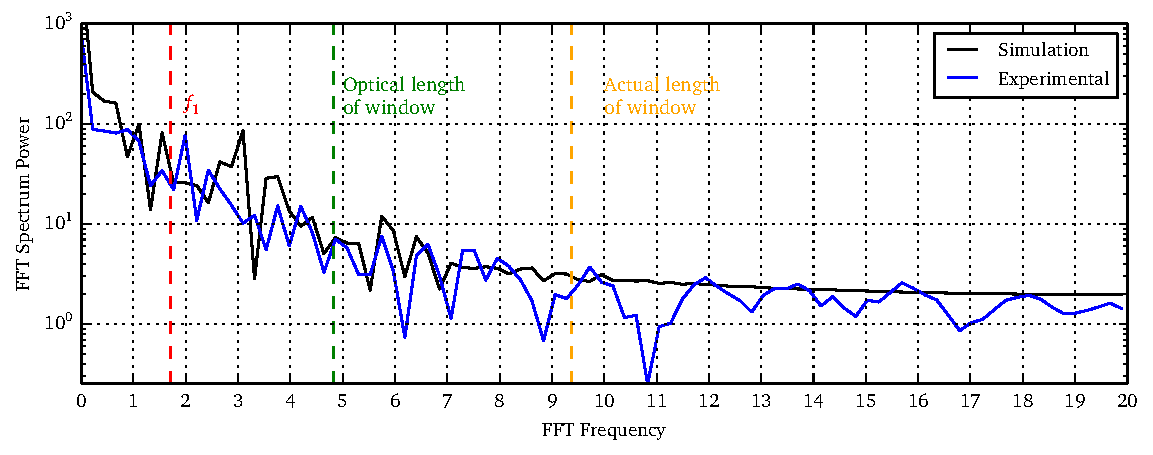
\includegraphics[width=0.8\textwidth]{figs/active/fourierAnalysisS11.pdf}
 \caption[Fourier Power Spectrum]
	  {Absolute value of the Fourier transform of the $S_{11}$ parameter.
	  The red lines denote the frequencies associated with certain lengths
	  in the RF21 fibre design.}
 \label{fig:antenna.fourierAnalysis}
\end{figure}



% \section{Antenna Propagation}
% 
% \todo[inline]{Describe goal of project; advantages of using fibers
% 	      over patch antennae...}
% 	      
% \subsection{Antenna Theory Primer}
% \todo[inline]{Basic definitions of directivity, gain...}
% \todo[inline]{Stratton solution}
% 
% \subsection{Designs}
% 
% \todo[inline]{Feasability of design via dipole antenna. Analytical solution
% 	      of dipole antenna. Issue with thin silver shells.}
% 
% \todo[inline]{Theory of infinite LCXs as guide for finite LCX. Discuss in more
% 	      detail about the thin silver shells (methods used to model them,
% 	      non-agreement with experimental data and its probable causes).
% 	      Discuss Bruggemann's model and Fuchs-Sondheimer methods.}